% SNAS 2026 camera-ready short paper.
% Built on the official SNAS_main.tex camera-ready template distributed by the
% program committee on 2026-09-15. Package list, spacing, title block, and
% caption setup follow that template; the \newcolumntype{L} table helper and
% the hyperref metadata below are the only additions this manuscript needs.
% Compile with: pdflatex -> bibtex -> pdflatex -> pdflatex

\documentclass[12pt,letterpaper]{article}

\usepackage[margin=1in]{geometry}

% Times New Roman-like font
\usepackage{newtxtext}
\usepackage{newtxmath}

\usepackage{abstract}

% APA-style citations, drawn from references.bib via BibTeX
\usepackage[natbibapa]{apacite}

\usepackage{setspace}
\onehalfspacing

\usepackage{microtype}

\usepackage{titlesec}
\titlespacing*{\section}{0pt}{0.6\baselineskip}{0.3\baselineskip}
\titlespacing*{\subsection}{0pt}{0.45\baselineskip}{0.2\baselineskip}
\titlespacing*{\subsubsection}{0pt}{0.35\baselineskip}{0.15\baselineskip}

\usepackage{graphicx}

\usepackage{booktabs}
\usepackage{multirow}
\usepackage{array}
\usepackage{tabularx}
\usepackage{makecell}
\usepackage{colortbl}

% Ragged-right fixed-width column used by this manuscript's tables.
\newcolumntype{L}[1]{>{\raggedright\arraybackslash}p{#1}}

\usepackage{amsmath}
% newtxmath already defines \Bbbk, so loading amssymb after it is a fatal
% "command already defined" error. The official template ships both packages in
% this order and so hits this; undefining the symbol first lets amssymb supply
% its own without changing anything the template renders.
\let\Bbbk\relax
\usepackage{amssymb}
\usepackage{amsfonts}
% Same collision, second instance: newtxmath supplies \openbox and the proof
% environment, which amsthm then tries to define again.
\let\openbox\relax
\let\proof\relax
\let\endproof\relax
\usepackage{amsthm}

\usepackage{textcomp}
\usepackage{url}
\usepackage{placeins}
\usepackage{enumitem}
\usepackage{xcolor}

\raggedbottom

% Compression: keep floats from opening large vertical gaps.
\setlength{\textfloatsep}{8pt plus 2pt minus 2pt}
\setlength{\floatsep}{6pt plus 2pt minus 2pt}
\setlength{\intextsep}{6pt plus 2pt minus 2pt}

\usepackage[hidelinks,bookmarks=true]{hyperref}
\hypersetup{
  pdftitle={ConstructionSafety-FaithBench: Evaluating Visual-Evidence Sensitivity in Construction-Safety Vision-Language Systems},
  pdfauthor={Md Kamruzzaman, Eashraque Jahan, Mustafa Abdallah},
  pdfsubject={SNAS 2026 camera-ready short paper},
  pdfkeywords={trustworthy AI, explainable AI, vision-language models, construction safety, evidence sensitivity}
}

\newtheorem{definition}{Definition}
\newtheorem{example}{Example}
\newtheorem{theorem}{Theorem}

\usepackage{caption}
\captionsetup{font=small,labelfont=bf,labelsep=period}

\renewcommand{\arraystretch}{1.15}

% ---- Author / affiliation commands (verbatim from SNAS_main.tex) ----
\newcommand{\Author}[2]{%
    #1$^{#2}$%
}
\newcommand{\Affiliation}[2]{%
    $^{#1}$#2
}

\makeatletter
\renewcommand{\maketitle}{
    \begin{center}
        {\fontsize{16}{19}\selectfont
        \bfseries
        \@title\par}
        \vspace{8pt}
        {\fontsize{12}{14}\selectfont
        \@author\par}
    \end{center}
    \vspace{6pt}
}
\makeatother

\date{}

\begin{document}

% apacite spells out every author the first time a 3-to-5-author work is cited.
% The pre-port manuscript used "et al." throughout, which is also APA 7, so force
% the short form for the multi-author entries.
\shortcites{li2025rationales,villa2025merlim,wu2024faithfulness,xiao2024florence}

\title{
    \vspace{-1.0cm}
    \fontsize{16}{19}\selectfont
    \bfseries
    ConstructionSafety-FaithBench: Evaluating Visual-Evidence Sensitivity
    in Construction-Safety Vision-Language Systems
}

\author{
    \Author{Md Kamruzzaman}{1,*};
    \Author{Eashraque Jahan}{2};
    \Author{Mustafa Abdallah}{1}
    \\[4pt]
    \Affiliation{1}{
        Purdue University, West Lafayette, IN, United States
    }
    \\
    \Affiliation{2}{
        University of Denver, Denver, CO, United States
    }
    \\[4pt]
    kamrul28890@gmail.com;
    easha003eee@du.edu;
    abdalla0@purdue.edu
    \\[2pt]
    $^{*}$Corresponding author
}

\maketitle

\vspace{-0.6cm}

\begin{abstract}

Construction safety depends on small, rule-specific visual details: a hard hat on a particular worker, a barrier at a particular edge. Vision-language models (VLMs) are increasingly proposed to check such details automatically, but they can give the right safety answer for the wrong visual reason, judging a scene unsafe because construction sites look hazardous while ignoring the cue the rule concerns. Existing evaluations report answer accuracy and are silent on this failure. We introduce ConstructionSafety-FaithBench, an audit benchmark that separates three properties usually merged into one score: whether the answer is correct, whether the cited visual evidence is rule-relevant, and whether the answer changes when that evidence is removed. Evidence dependence is probed by occluding the rule-relevant region and comparing the effect against occlusions of identical size placed elsewhere in the image, so any difference reflects location rather than the amount removed. The benchmark is model-agnostic; here we validate it on one system, an open-vocabulary grounding pipeline built on Florence-2, across hard-hat, fall-protection, guardrail, and struck-by rules. For that system the three properties come apart. The pipeline reaches 18.3\% accuracy on 120 adjudicated hard cases. It returns an evidence region on 98.8\% of images, yet those regions overlap the rule-relevant one poorly, mean intersection-over-union 0.058. It nonetheless flips its answer 39.2\% of the time under targeted occlusion, against 9.2\% under size-matched random occlusion, a paired difference of 30.0 points. It never answers ``uncertain,'' even where a single frame cannot support a decision. Coming from one system on one imagery source, these findings characterize that pipeline rather than vision-language models in general. They nonetheless indicate that answer accuracy is insufficient evidence of trustworthiness for safety-critical screening, and that a system's willingness to abstain deserves scrutiny alongside its accuracy. Benchmark, code, and frozen artifacts: \url{https://github.com/kamrul28890/snas-2026-construction-safety-faithbench}.

\end{abstract}

\vspace{2pt}

\noindent
\textbf{Keywords:}
trustworthy AI; explainable AI; vision-language models;
construction safety; evidence sensitivity

\section{Introduction}

Construction and extraction occupations accounted for 1,032 fatal work injuries in the United States in 2024, of which 370 were falls, slips, and trips \citep{bls2026cfoi}; regulators group the leading causes of construction death into falls, struck-by incidents, caught-in or caught-between events, and electrocution \citep{osha_focusfour}. Most of these hazards are visible in the moments before they cause harm, so safety supervision is largely a visual task: a supervisor looks at a specific worker, edge, or machine and decides whether a specific written rule is being followed. The limiting factor is coverage, and sites already produce large volumes of imagery from fixed cameras, drones, and routine documentation that could be checked automatically against those rules.

Vision-language models (VLMs), which take an image together with a natural-language prompt and return a natural-language response, are an appealing tool for this, and some can additionally return the image regions they associate with that response. Because the rule is expressed in text rather than trained into a fixed classifier, one model can be asked about hard hats today and guardrails tomorrow without retraining. But safety-critical use changes what counts as an acceptable answer: a missed fall-protection violation can precede a fatal fall, and a confidently reported hazard that does not exist erodes the trust that makes the tool usable at all. It is not enough to be right on average. A reviewer needs to know whether a particular verdict rests on the visual evidence the rule actually concerns.

Existing evaluation does not close this gap. Benchmarks for construction-safety VLMs report answer accuracy, which measures correctness but is silent on whether the answer used the right evidence \citep{chen2025inspectors}, and broader multimodal work on rationale quality is not specific to safety rules or to the localized, object-level cues they depend on \citep{li2025rationales}. Most directly, MERLIM identifies \textit{hidden hallucinations}, correct answers produced without meaningful visual grounding, reporting that instruction-tuned models often succeed by exploiting global scene patterns and language priors rather than the visual content in question \citep{villa2025merlim}. That work establishes the phenomenon on general imagery; it does not test whether the same failure occurs when a written rule designates which region is decisive, which is the situation a safety inspection creates. Methodologically, explanation-faithfulness research has repeatedly shown that internal scores such as attention weights can look convincing while failing to track what a model uses \citep{jain2019attention,wu2024faithfulness}, motivating tests of behavior under controlled intervention and aligning with the descriptive-accuracy and robustness requirements set out for explainable systems \citep{phillips2021principles}.

This paper addresses that gap by separating three properties that a single accuracy score merges. They come apart in practice: a system can be correct without being grounded, by inferring ``unsafe'' from generic construction-scene clutter, and it can return a plausible-looking region without that region driving its answer. We therefore ask three questions:

\begin{itemize}
\item \textbf{RQ1 (Correctness).} How accurately does the evaluated grounding pipeline answer construction-safety rule questions, scored against adjudicated reference labels?
\item \textbf{RQ2 (Evidence relevance).} Does the visual evidence the pipeline returns correspond to the region the safety rule actually concerns?
\item \textbf{RQ3 (Intervention sensitivity).} Does removing the rule-relevant region change the pipeline's answer more than removing an equally sized region elsewhere in the same image?
\end{itemize}

We are deliberately careful about how these three relate to \textit{faithfulness}, the stronger property that a system's answer genuinely depends on the evidence that ought to support it. They contribute evidence toward such an assessment without establishing it. Intervention sensitivity in particular is necessary but not sufficient: an answer that changes when rule-relevant pixels are removed shows dependence on that location, yet a black rectangle also introduces an artifact the system may react to, and an answer that does \textit{not} change may reflect redundant cues or language priors rather than an absent dependence. We therefore report sensitivity as an observable behavior and treat faithfulness as an interpretive question this evidence informs without resolving.

To answer them we introduce ConstructionSafety-FaithBench, a compact and reproducible audit benchmark whose every example pairs a construction-site image with a written safety rule, an answer label, the evidence regions the rule depends on, and provenance fields recording where each label came from. It covers four rule families matched to the leading hazard categories: harness and fall protection and guardrail and edge protection, both addressing falls; struck-by hazards from equipment proximity; and hard-hat and personal protective equipment (PPE) compliance, the principal control against head injury.

The schema, metrics, and intervention protocol are model-agnostic, and any system that accepts an image and a written rule and returns an answer with evidence regions can be run through them. The empirical results, by contrast, come from a single system, so findings are phrased throughout as properties of the evaluated pipeline rather than of the model class. These are evaluation contributions: the study audits an existing system rather than proposing a new one, and describes measurement, not deployment readiness.

\section{Benchmark and Audit Pipeline}

\subsection{Images and Safety Rules}

The benchmark is built from ConstructionSite imagery and its metadata, a collection released with safety-oriented captioning, rule-violation, and object-grounding annotations \citep{chen2025inspectors}, chosen because it provides real construction scenes with the safety-relevant object annotations a rule-level audit requires; generic object-detection corpora do not carry safety semantics. Each row pairs one image with one written safety rule and records an image identifier, the source split, the safety question in natural language, a normalized rule identifier, the answer label, the evidence regions the rule depends on as \textit{bounding boxes} in pixel coordinates, and provenance metadata describing where the label came from.

Answers use three labels: \textit{compliant}, \textit{violation}, and \textit{uncertain}, the last meaning the image does not contain enough information to decide. The third matters for safety review, because a system forced to choose between the first two will guess when it should defer. A 163-row pilot split supports the intervention study and a 588-row scale-up split tests whether the pipeline behaves consistently at larger scale. Raw images and model weights are not redistributed; the released scripts load source images only when the user already has local dataset access.

\subsection{The Evaluated Pipeline}

The system under audit answers a safety question in two steps: it locates candidate objects, then applies a fixed rule to those locations to produce a verdict. The locating step uses the \textit{microsoft/Florence-2-base-ft} release of Florence-2, a compact vision-language model that accepts an image with a text prompt and returns bounding boxes for the objects that prompt describes \citep{xiao2024florence}. This capability is called \textit{open-vocabulary grounding}: the model is not restricted to a fixed list of trained categories, so it can be asked for ``hard hat'' or ``guardrail'' directly, in words, without retraining for each new rule. We selected it because it is small enough to run repeatedly on modest hardware, which the intervention study requires.

Around it we build a \textit{grounding adapter}, a thin wrapper that prompts Florence-2 for the objects a rule concerns and applies fixed geometric tests to the returned boxes; a hard-hat rule, for example, checks whether a helmet box overlaps the head region of each detected worker. These tests are \textit{deterministic}, involving no learned parameters and no randomness, so that any failure can be traced to either the grounding step or the rule logic rather than hidden inside a second black box.

Three reference points require no image understanding at all and bound the problem from below. A \textit{manifest-seed} baseline echoes the label already stored in the manifest, revealing how much of the annotation is circular; a \textit{majority-violation} baseline always answers ``violation,'' establishing the score obtainable from class imbalance alone; and a \textit{caption-keyword} baseline reads only the text caption, testing whether captions leak the answer.

\subsection{From Image to Score}

Figure~\ref{fig:pipeline} summarizes the full path from image and rule to the three scores. Every stage writes normalized CSV and JSONL records, so each reported number can be traced back to the run that produced it.

\begin{figure}[t]
\centering
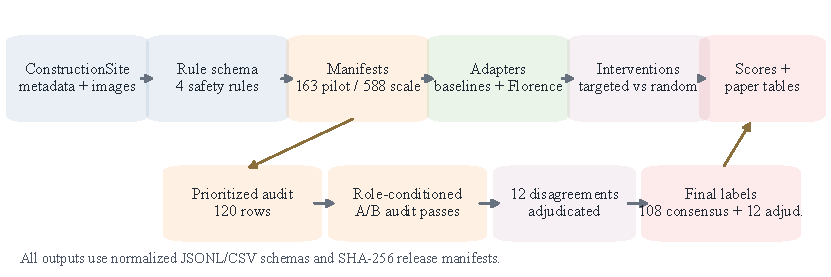
\includegraphics[width=\linewidth]{figures/pipeline_architecture.pdf}
\caption{The ConstructionSafety-FaithBench evaluation pipeline. Construction images and written safety rules are converted into benchmark manifests, answered by the evaluated adapters, audited into final labels, and subjected to targeted and size-matched random occlusions, yielding the correctness, grounding, and faithfulness scores reported in Section 4.}
\label{fig:pipeline}
\end{figure}

\subsection{The Audit Label Layer}

Scoring requires reference labels, and their quality bounds what the evaluation can claim. The benchmark builds them in three layers. Automated baseline annotations derived from the dataset's own metadata scale cheaply, but come from the same metadata used to assemble the splits, so they are never treated as independent ground truth. A prioritized audit set of 120 rows is then drawn by conditioning on disagreement between the pipeline and that baseline, which is where expensive adjudication is most informative; 118 of the 120 are outright answer disagreements. \textbf{The audit set is therefore enriched for disagreement and is not a representative sample.} Statistics computed on it estimate performance on contested cases, not across the benchmark, so every audit-set figure below is reported alongside the corresponding figure from the full 163-row pilot and 588-row scale-up splits. Finally, every audited row receives two independent passes, with the 12 disagreements resolved by a returned adjudication step. The passes agree on 108 of 120 rows, but raw agreement flatters a set in which one label dominates, so we report Cohen's $\kappa = 0.78$ against an expected agreement of 0.54. That is substantial consistency in applying the protocol; it does not establish that the protocol is correct, because both passes were generated by AI annotators working from the same written instructions rather than by independent human domain experts.

We therefore call the result \textit{reference labels} rather than ground truth. The task mixes perceptual judgments a careful non-expert can answer reliably, such as whether a helmet is visible on a given head, with safety judgments that depend on training and site experience, such as whether a given proximity to operating equipment is unsafe; only the first is well supported by our procedure. The six rows adjudicated \textit{uncertain} concentrate in exactly the judgment-dependent cases, such as a static frame that cannot establish an excavator's swing radius. That these labels have not been validated by independent construction-safety professionals is the single largest threat to the validity of every accuracy figure we report.

\section{Metrics and Experimental Setup}

Each research question requires a different measurement, and the central design decision of this benchmark is to keep them apart. The three subsections below define the metrics for RQ1, RQ2, and RQ3 in turn, and Section~\ref{sec:results} reports each in the same order.

\subsection{Answer Metrics (RQ1)}

\textit{Accuracy} is the proportion of rows where the pipeline's answer matches the audit label. It is misleading under class imbalance: because most audited rows are violations, a system that always answers ``violation'' scores well without understanding anything. \textit{Macro-F1}, the equally weighted average of the per-class F1 scores for compliant, violation, and uncertain, corrects for this, so a model handling only the majority class scores high on accuracy and low on macro-F1. Both are reported as percentages and higher is better; the gap between them is diagnostic of a system exploiting the label distribution rather than reading the image.

\subsection{Evidence Metrics (RQ2)}

\textit{Evidence presence} records whether the pipeline returned any region at all, which matters because a system that silently returns nothing cannot be audited and an unexplained verdict is not actionable. \textit{Box overlap} compares the returned region with the rule's reference region using intersection over union (IoU), the area two rectangles share divided by the area they jointly cover, where 1.0 means they coincide and 0 that they do not touch. \textit{Normalized centroid drift} measures how far the center of the returned region moves as a fraction of the image diagonal, so the number is comparable across image sizes. We report drift alongside IoU because the two disagree systematically on small objects: for a small hard hat a modest shift destroys IoU while barely moving the centroid, so IoU alone would overstate the instability.

\subsection{Intervention Metrics (RQ3)}
\label{sec:intervention}

Faithfulness cannot be read off a single run, because a correct answer and a well-placed box are both compatible with the model ignoring the evidence entirely. We therefore intervene on the image and observe what changes.

For each image a \textit{targeted occlusion} places a solid black rectangle over the first rule-relevant object box recorded in the manifest: the worker and head region for hard-hat rows, the exposed edge or barrier for guardrails, the worker-at-height region for fall protection, and the worker and equipment proximity region for struck-by risk. If the model is genuinely using that evidence, removing it should change the verdict or push it toward uncertainty. Each matched-random control uses the identical clipped width and height at a seeded random location chosen to keep target overlap at or below 0.05 IoU, falling back to the lowest-overlap candidate and reporting the resulting overlap rather than discarding the image. Five controls per image give 948 runs in total: 158 targeted occlusions and 790 controls.

Any occlusion changes the image, so a change in answer proves nothing on its own; the control is what makes this a test rather than an observation. Because the number of occluded pixels is held constant, a systematic difference between conditions cannot be attributed to the amount removed. Table~\ref{tab:maskchar} confirms the size match holds exactly and characterizes what else differs.

\begin{table}[h]
\centering
\caption{Occlusion characteristics by condition. Mask area is identical by construction, so the conditions differ in placement rather than extent. Areas are strongly right-skewed, hence both mean and median. The last row shows the limitation discussed below.}
\label{tab:maskchar}
{\setstretch{1.0}\small
\begin{tabular}{L{1.45in}rr}
\toprule
Quantity & Targeted & Matched-random \\
\midrule
Occlusions & 158 & 790 \\
Mask area, mean share & 0.136 & 0.136 \\
Mask area, median share & 0.014 & 0.014 \\
Mask--target IoU & 1.000 & 0.056 \\
Mask area on target & 100.0\% & 7.1\% \\
Removed worker detection & 5.1\% & 1.4\% \\
\bottomrule
\end{tabular}
\par}
\end{table}

The control isolates less than it may appear. It does establish that the effect is not produced by removing pixels as such, since 88.2\% of random masks overlap the target at an IoU of 0.05 or below while occluding an identical area. It does not establish that the rule-relevant region is special among \textit{informative} regions, because a randomly placed mask disturbs content the pipeline was actually using only 1.4\% of the time, against 5.1\% for targeted masks: the comparison separates rule-relevant evidence from arbitrary image area, not from other meaningful content. A near-target control, placing an equally sized mask adjacent to but not overlapping the rule region, is the most valuable single extension to the protocol. Mask areas are also strongly right-skewed, and on the 13 of 158 targets covering more than half the image the control is geometrically degenerate, since an equally sized mask cannot avoid a box that large; their random masks average a target IoU of 0.572 with none reaching the criterion, against 0.009 and a 96.1\% success rate on the remaining 145. We therefore repeat the primary comparison with those images removed and report both results. Finally, a black rectangle is not a natural occlusion, and size matching controls for that artifact only to the extent that both conditions introduce an identical one.

The primary statistic is the \textit{answer-flip rate}, the proportion of images whose answer changes after occlusion, reported as a paired difference defined per image as the targeted outcome minus the mean of that image's five controls; pairing within image removes differences in scene difficulty. A difference near zero would indicate no more sensitivity to rule-relevant evidence than to arbitrary pixels, a large positive difference location-specific dependence. Confidence intervals come from image-level bootstrap resampling with 10{,}000 resamples, and paired comparisons use the two-sided Wilcoxon signed-rank test with matched-pairs rank-biserial correlation as the effect size and Holm correction across the two primary paired tests.

The full configuration of the intervention study, covering model and dataset revisions, decoding settings, mask construction, placement search, seeds, and every statistical setting quoted above, is frozen in \texttt{analysis/protocol.json} in the released repository and is reproduced in the repository documentation.

Using this protocol, we now compare the evaluated pipeline in terms of answer performance, evidence quality, and evidence dependence.

\section{Results}
\label{sec:results}

We report each research question in turn. Table~\ref{tab:headline} collects the headline quantities; the subsections that follow explain what each one means.

\begin{table}[h]
\centering
\caption{Headline results. The first block describes the audited evaluation set, the second answers RQ1 (correctness) and RQ2 (evidence relevance), the third breaks RQ1 down by safety-relevant error direction, and the fourth answers RQ3 (intervention sensitivity). For accuracy, macro-F1, and evidence presence, higher is better; for the paired differences, larger values indicate stronger dependence on rule-relevant evidence. A missed violation is a genuine violation reported as compliant. Because the audit set is enriched for disagreement, the error rates describe contested cases and overstate what would occur across the full splits.}
\label{tab:headline}
{\setstretch{1.0}
\begin{tabular}{lr}
\toprule
Quantity & Value \\
\midrule
Final audit rows & 120 \\
Final audit label counts & 83 V / 31 C / 6 U \\
A/B agreement rows & 108 \\
Returned adjudication rows & 12 \\
\addlinespace
Florence-2 accuracy on audit labels & 18.3\% \\
Florence-2 macro-F1 on audit labels & 12.5\% \\
Automated baseline accuracy on audit labels & 78.3\% \\
Florence-2 evidence presence (scale-up) & 98.8\% \\
Florence-2 mean best evidence IoU (scale-up) & 0.058 \\
\addlinespace
Florence-2 missed violations & 70/83 (84.3\%) \\
Florence-2 false alarms & 22/31 (71.0\%) \\
Metadata baseline missed violations & 11/83 (13.3\%) \\
Metadata baseline false alarms & 9/31 (29.0\%) \\
\addlinespace
Targeted answer-flip rate & 39.2\% \\
Matched-random answer-flip rate & 9.2\% \\
Paired answer-flip difference & 30.0 points \\
Paired centroid-drift difference & 0.166 \\
\bottomrule
\end{tabular}
\par}
\end{table}

\subsection{Answer Correctness (RQ1)}

The key comparison in Figure~\ref{fig:audit} is between the automated baseline and the grounding pipeline on the same 120 adjudicated rows. The automated baseline reaches 78.3\% accuracy, but this number should not be read as competence. That baseline is derived from the same dataset metadata used to assemble the candidate split, so it is partly scoring itself. Its macro-F1 of 50.5\% exposes the difference: it handles the majority violation class and fails elsewhere.

Florence-2 reaches 18.3\% accuracy and 12.5\% macro-F1 on this set. Two caveats keep this from being a general performance claim. First, the audit set was deliberately built from disagreement and weak-overlap cases, so it represents hard cases rather than average ones. On the full splits scored against the weaker metadata-assisted labels, the same pipeline reaches 41.7\% accuracy on the 163-row pilot and 39.3\% on the 588-row scale-up. Second, the low audit-set score is a statement about the complete pipeline, grounding plus rule logic, not about Florence-2's detection ability in isolation.

Accuracy is the wrong summary for a safety task, because it prices a missed hazard and a false alarm identically. The third block of Table~\ref{tab:headline} separates them. On these contested rows the pipeline reported \textit{compliant} for 70 of the 83 genuine violations, a missed-violation rate of 84.3\%, while also raising false alarms on 22 of 31 compliant rows. Both directions are poor, but they are not equally consequential: a false alarm costs an unnecessary inspection, whereas a missed violation is the failure the system exists to prevent. For comparison, the metadata-assisted baseline misses 13.3\% of violations on the same rows.

Two further patterns matter more than the headline number. The pipeline never returned \textit{uncertain} on any of the 120 audited rows, despite six rows being adjudicated as genuinely undecidable from a single frame. On the hard-hat and guardrail slices it went further and answered \textit{compliant} for all 30 rows in each, even though 26 and 24 of those rows respectively were violations. A system that cannot abstain and cannot flag a violation in an entire rule family is not merely inaccurate; it fails silently, in the direction that matters most for safety.

For comparison, three strategies that never look at the image at all provide the floor. A manifest-seed baseline that echoes the stored label scores 100\% by construction, confirming that portion of the annotation is circular. A majority-violation baseline that always answers ``violation'' reaches 69.3\% on the pilot and 57.5\% on the scale-up split. A caption-keyword baseline that reads only text reaches 19.7\%, which shows the labels are not simply recoverable from captions. The relevant lesson is that answering ``violation'' every time outperforms the grounding pipeline on these splits, so accuracy alone cannot demonstrate that a model is reading the image.

\begin{figure}[t]
\centering
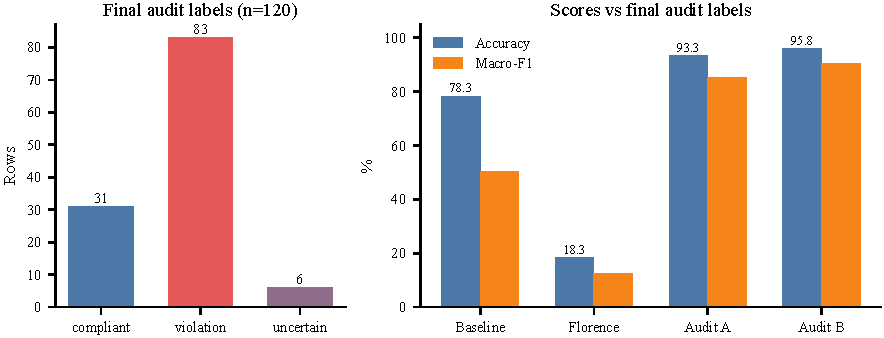
\includegraphics[width=0.82\textwidth]{figures/audit_result_dashboard.pdf}
\caption{Composition of the 120-row adjudicated audit set (left) and answer scores against those labels (right). The audit split deliberately over-samples disagreement and weak-overlap cases, so these accuracies describe hard cases rather than average-case performance.}
\label{fig:audit}
\end{figure}

\subsection{Evidence Quality (RQ2)}

Correctness scores say nothing about whether the pipeline pointed at the right thing. Table~\ref{tab:rulelevel} answers that question, and the pattern to look for is the gap between accuracy and evidence presence within each rule family.

The pipeline almost always produces evidence: it returned at least one region for 96.9\% of pilot rows and 98.8\% of scale-up rows. The regions themselves, however, agree poorly with the rule's reference region. Mean best IoU is 0.369 on the pilot split and only 0.058 on the scale-up split. An IoU of 0.058 means the returned rectangle and the rule-relevant rectangle barely intersect.

The rule-level breakdown in Table~\ref{tab:rulelevel} explains the difference between the two splits and is itself the more informative result. Hard-hat rows dominate the scale-up split, 303 of 588, and carry the worst overlap at 0.030. Struck-by rows are similar at 0.033. These are exactly the rule families whose evidence is small or relational: a hard hat occupies a few dozen pixels on a worker's head, and equipment proximity is a relationship between two objects rather than a single object with a boundary. Guardrail and fall-protection evidence is physically larger, and overlap is correspondingly better at 0.171 and 0.130.

\begin{table}[h]
\centering
\caption{Scale-up split by rule family. Evidence presence is near-total in every family, while overlap with the rule-relevant region is weak, especially where the evidence is small (hard hat) or relational (equipment proximity). Higher is better in all columns.}
\label{tab:rulelevel}
{\setstretch{1.0}\small
\begin{tabular}{L{1.35in}rrrr}
\toprule
Rule family & $n$ & Accuracy & Evid.\ present & Mean IoU \\
\midrule
Fall / harness & 69 & 59.4\% & 98.6\% & 0.130 \\
Guardrail / edge & 110 & 63.6\% & 96.4\% & 0.171 \\
PPE / hard hat & 303 & 30.7\% & 99.3\% & 0.030 \\
Struck-by / equipment & 106 & 25.5\% & 100.0\% & 0.033 \\
\midrule
Overall & 588 & 39.3\% & 98.8\% & 0.058 \\
\bottomrule
\end{tabular}
\par}
\end{table}

The practical consequence is specific. A safety reviewer using this pipeline would receive a bounding box on essentially every image, which looks like a system that always shows its work. On hard-hat rows that box would usually not contain the hard hat in question. Evidence presence is therefore not evidence quality, and an interface that displays model evidence without scoring it can create confidence that the underlying measurement does not support.

\subsection{Evidence Dependence (RQ3)}

The final question is whether the answer depends on the rule-relevant region at all. The comparison to read in Figure~\ref{fig:intervention} is targeted occlusion against size-matched random occlusion, since both remove identical numbers of pixels.

Occluding the rule-relevant region changed the answer 39.2\% of the time, against 9.2\% for size-matched random masks. The paired difference is 30.0 percentage points, with a bootstrap 95\% interval of 22.3 to 37.7 points and a rank-biserial effect size of 0.89. Evidence relocation shows the same pattern: the paired centroid-drift difference is 0.166, interval 0.140 to 0.193, Holm-adjusted $p < .001$.

Because the control degenerates on the 13 images whose target box covers more than half the frame, we repeat the comparison without them. The difference does not depend on those cases; it grows slightly, to 31.7 points with an interval of 23.7 to 39.9 across the remaining 145 images. This is the expected direction, since on degenerate images the ``random'' mask substantially overlaps the target and therefore flips answers too, compressing the gap. We report the pooled figure as the headline result because it is the more conservative of the two.

This cuts both ways. The model is not merely reacting to generic construction-scene clutter: were it doing so, the paired difference would sit near zero, and it does not. But sensitivity is not sound reasoning. When rule-relevant evidence disappears, the appropriate response for a safety system is to report that it can no longer tell; instead the pipeline substitutes a different confident verdict, consistent with the complete absence of \textit{uncertain} answers under RQ1. In a deployed screening tool, an occluded, dirty, or badly angled view of a worker would not produce a flag for human review but a different answer, delivered with the same confidence as the original.

The three results are therefore not redundant: the pipeline is often wrong (RQ1), usually points somewhere unhelpful (RQ2), and is nonetheless measurably sensitive to the right pixels (RQ3). Any one measured alone would mislead.

\begin{figure}[t]
\centering
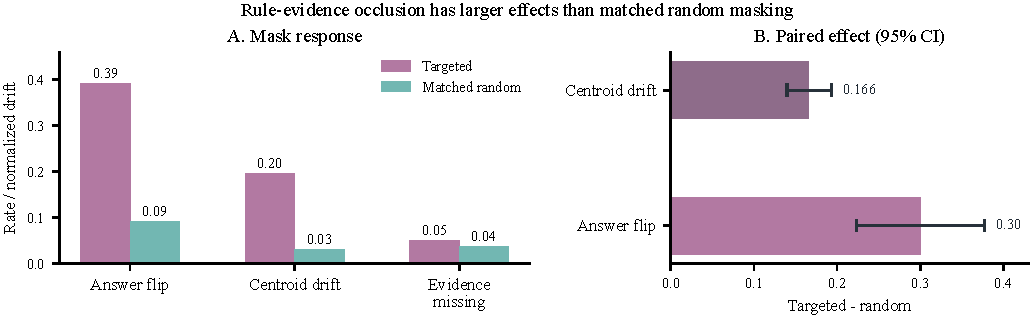
\includegraphics[width=0.82\textwidth]{figures/intervention_effects_chart.pdf}
\caption{Effect of occluding rule-relevant evidence compared with occluding an equally sized random region in the same image. Because both conditions remove the same number of pixels, the difference between them isolates the contribution of location rather than disruption.}
\label{fig:intervention}
\end{figure}

\subsection{Qualitative Cases}

Two audit rows show what these aggregates look like in practice. In a PPE row labelled a violation, a third pedestrian in dark clothing is bare-headed while nearby workers wear yellow hard hats; a system drawn to the salient helmets records compliance and misses the person actually at risk. In a struck-by row, a worker stands near an operating excavator and the single frame cannot confirm distance or swing state, precisely the situation an \textit{uncertain} answer exists to express. Both share a structure: the correct judgment depends on a small, rule-defined region while the surrounding image offers abundant cues pointing toward a plausible but unfounded answer.

\section{Discussion and Implications}

The central finding is that correctness, grounding, and evidence dependence dissociate. A benchmark reporting only the first would call this system weak; one reporting only the third would call it evidence-driven. Both descriptions would be incomplete, and the safety-relevant behavior sits in the disagreement between them.

A plausible explanation lies in the difference between detecting an object and adjudicating a rule. Open-vocabulary grounding is trained to answer ``where is X,'' whereas a safety rule asks whether every worker in view satisfies a requirement, a quantified judgment that often turns on \textit{absence}: no hard hat on that head, no barrier at that edge. A detector that fails to find an object cannot distinguish that failure from the object being absent, so the rule logic must adopt a default verdict for ungrounded cases, and that default then answers every case where grounding fails. This is consistent with the degenerate all-compliant behavior on the hard-hat and guardrail slices, precisely the families with the weakest evidence overlap.

The implication for construction safety concerns failure mode rather than accuracy alone. A screening tool that misses hazards is dangerous; one that misses them while displaying a confident verdict and a plausible bounding box is worse, because it supplies the visual trappings of justification. A reviewer would receive a box on 98.8\% of images, and on hard-hat rows that box would usually not contain the relevant hard hat. The safety-relevant property is not only how often a system is right, but whether it knows when it cannot tell. Two recommendations follow: evaluations of safety-critical VLMs should report an abstention rate alongside accuracy, treating a system that never returns ``uncertain'' as unvalidated for review support; and displayed evidence regions should be scored rather than merely rendered, since unscored evidence invites reviewers to assume a grounding that has not been demonstrated.

These findings extend to a safety-critical visual domain the established results that plausible-looking explanations need not reflect what a model uses \citep{jain2019attention,wu2024faithfulness} and that correct answers can be produced without visual grounding at all \citep{villa2025merlim}. Our addition is the rule-defined reference region: where hidden hallucinations have previously been identified against general visual content, a safety rule specifies in advance which region should be decisive, which makes the targeted intervention well posed. They also qualify optimism about applying general-purpose VLMs to construction inspection \citep{chen2025inspectors}, since our pipeline's difficulty is not primarily detection but the translation from detections into rule verdicts, which is where safety semantics live.

\section{Threats to Validity and Limitations}

\textbf{Model coverage.} One system was evaluated, so every empirical statement here describes that pipeline. We cannot separate failures specific to Florence-2 from failures of compact grounding models generally, or of the detection-to-rule translation any such pipeline requires; comparative claims need a wider model suite.

\textbf{Selection.} The audit set conditions on pipeline--baseline disagreement, so its statistics describe contested cases rather than the benchmark as a whole. Full-split figures accompany every audit-set figure for this reason, but the enrichment cannot be undone analytically, and a subset sampled without conditioning on disagreement would be a stronger design.

\textbf{Annotation.} Reference labels come from two AI passes plus adjudication, not from independent construction-safety professionals. The safety-judgment portion of the task, as distinct from the perceptual portion, is least supported by that procedure and determines most reported accuracies.

\textbf{Intervention and control.} As Section~\ref{sec:intervention} sets out, a black rectangle is not a natural occlusion, and size matching equalizes but does not eliminate the artifact. The controls separate the rule-relevant region from arbitrary image area rather than from other informative content, and they degenerate entirely on the 13 images with very large targets, which is why the comparison is also reported with those images excluded.

\textbf{Interpretation.} Intervention sensitivity is an observable behavior, not a demonstration of faithful reasoning. A changed answer shows dependence on the occluded location, not reasoning from that evidence in any richer sense; an unchanged answer is equally ambiguous, since redundant visual cues, language priors, or an ineffective mask would each produce one.

\textbf{Scope of measurement.} The benchmark does not measure human-like reasoning, internal chain-of-thought, causal reasoning in any strong sense, general interpretability, deployment reliability, real-world injury reduction, or how human reviewers respond to displayed evidence. It measures three observable behaviors on a fixed set of images and rules and supports comparison between systems evaluated under the same protocol; it is one mechanism within a broader trustworthy-AI evaluation programme, not such a programme on its own.

\textbf{Scale and distribution.} Coverage is 163 pilot and 588 scale-up rows from a single source collection, sharply imbalanced: scanning 3,004 source rows yielded only 13 struck-by-risk and 75 fall-hazard candidates against 250 PPE-violation and 250 compliant. Struck-by and fall-hazard results are therefore diagnostic rather than stable estimates, and future releases should deliberately oversample rare but safety-critical events.

\textbf{Coverage of scenes and rules.} All imagery derives from one collection, so site types, regions, weather, lighting, and equipment conventions are not systematically varied, and four rule families stand in for safety programs that encompass many more, including electrical, confined-space, excavation, and housekeeping hazards. Every judgment is also made from a single frame, so hazards defined by motion or duration, such as equipment swing radius or how long a worker remains exposed, cannot be assessed; some rows are genuinely undecidable for this reason.

\textbf{Metric scope.} Evidence is compared at the level of rectangles, which does not capture whether the model used the correct part of a correctly located object.

\section{Ethical Considerations}

Construction imagery is imagery of people at work. A camera installed to check hard-hat compliance can equally support productivity monitoring, biometric identification, or retrospective review of an individual worker's conduct, and footage gathered for one purpose is routinely available for another. Safety monitoring does not by itself justify persistent worker surveillance; the two should be separated deliberately, through retention limits, restrictions on secondary use, meaningful consent, and worker representation in deployment decisions. The benchmark infers no identity, intent, competence, or blame, and should not be used for autonomous inspection or disciplinary monitoring: because the failure modes documented here fall hardest on missed violations, deploying such a system without human review would shift risk onto workers while presenting an appearance of oversight. Appropriate use is research evaluation under documented scope limits, data minimization, source-license compliance, and human professional review, consistent with risk-management guidance for AI-enabled workplace tools \citep{nist2023airmf,howard2024workplace}.

\section{Conclusion}

ConstructionSafety-FaithBench separates answer correctness, evidence grounding, and evidence dependence rather than collapsing them into one score. Auditing an open-vocabulary grounding pipeline across four construction rule families, we found the three come apart: 18.3\% accuracy on an adjudicated set of hard cases, an evidence region returned on 98.8\% of images but overlapping the rule-relevant region with mean IoU of 0.058, and answers that changed 39.2\% of the time under targeted occlusion against 9.2\% under size-matched controls. It never once answered ``uncertain.''

Answer accuracy is therefore insufficient evidence of trustworthiness in safety-critical visual applications, and faithfulness claims require interventions with size-matched controls rather than inspection of plausible-looking explanations. A screening tool's willingness to abstain deserves as much scrutiny as its accuracy, because the dangerous failure is not an obvious error but a confident verdict accompanied by evidence no one has scored. Replacing the AI-pass audit layer with domain-expert annotation, extending the model suite to stronger instruction-following VLMs, and testing how human reviewers respond to displayed evidence are the natural next steps.

\section*{Reproducibility Statement}

The benchmark, evaluation code, frozen model outputs, audit labels, intervention
specifications, score tables, and analysis scripts are at
\url{https://github.com/kamrul28890/snas-2026-construction-safety-faithbench}.
Every number reported here is regenerated from those artifacts by the included
scripts rather than transcribed by hand, and reproducing the reported statistics
and figures requires neither the source images nor a GPU. Images and model
weights are not redistributed; the scripts load images only where a local copy of
the ConstructionSite collection \citep{chen2025inspectors} is already available,
with the dataset revision recorded in each manifest row.

\label{bodyend}
\clearpage

\begingroup

\small

% APA reference list, generated from references.bib
\bibliographystyle{apacite}
\bibliography{references}

\endgroup

\end{document}
